\documentclass[10pt,letterpaper]{article}
\usepackage[top=0.85in,left=2.75in,footskip=0.75in]{geometry}

% Core maths/symbol packages
\usepackage{amsmath,amssymb}
\usepackage{textcomp,marvosym}

% Tables
\usepackage{changepage}
\usepackage[table]{xcolor}
\usepackage{array}
\usepackage{threeparttable}
\usepackage{adjustbox}
\usepackage{booktabs}

% Citations and hyperlinks
\usepackage{cite}
\usepackage{nameref,hyperref}

% Line numbers
\usepackage[right]{lineno}

% Typography
\usepackage[nopatch=eqnum]{microtype}
\DisableLigatures[f]{encoding = *, family = * }

% Captions
\usepackage[
  aboveskip=1pt,
  labelfont=bf,
  labelsep=period,
  justification=raggedright,
  singlelinecheck=off
]{caption}
\renewcommand{\figurename}{Fig}

% Header/footer
\usepackage{lastpage,fancyhdr,graphicx}
\usepackage{epstopdf}

% Remove brackets from bibliography numbering
\makeatletter
\renewcommand{\@biblabel}[1]{\quad#1.}
\makeatother

% Optional thick table rules from original template
\newcolumntype{+}{!{\vrule width 2pt}}
\newlength\savedwidth
\newcommand\thickcline[1]{%
  \noalign{\global\savedwidth\arrayrulewidth\global\arrayrulewidth 2pt}%
  \cline{#1}%
  \noalign{\vskip\arrayrulewidth}%
  \noalign{\global\arrayrulewidth\savedwidth}%
}
\newcommand\thickhline{%
  \noalign{\global\savedwidth\arrayrulewidth\global\arrayrulewidth 2pt}%
  \hline
  \noalign{\global\arrayrulewidth\savedwidth}%
}

% Layout
\raggedright
\setlength{\parindent}{0.5cm}
\textwidth 5.25in
\textheight 8.75in

\pagestyle{fancy}
\fancyhf{}
\rfoot{\thepage/\pageref{LastPage}}
\renewcommand{\headrulewidth}{0pt}
\renewcommand{\footrule}{\hrule height 2pt \vspace{2mm}}
\fancyheadoffset[L]{2.25in}
\fancyfootoffset[L]{2.25in}
\lfoot{\today}


\begin{document}
\vspace*{0.2in}
\begin{flushleft}

%    {\Large\textbf{\textit{EpiLink}: a label-free, process-based compatibility model for genomic transmission clustering in infectious disease surveillanc}}
    {\Large\bfseries\textit{EpiLink}: a label-free, process-based compatibility model for genomic transmission clustering in infectious disease surveillance}

%    Short: \textit{EpiLink}: process-based genomic transmission clustering



    \bigskip

    Dominic Arthur\textsuperscript{1},
    Christopher J. Banks\textsuperscript{1},
    Rowland R. Kao\textsuperscript{1,2*}

    \bigskip

    \textbf{1} The Roslin Institute, University of Edinburgh, Edinburgh, United Kingdom

    \textbf{2} School of Physics and Astronomy, University of Edinburgh, Edinburgh, United Kingdom

    \bigskip

    * rowland.kao@ed.ac.uk
\end{flushleft}

\section*{Abstract}
Identifying clusters of epidemiologically linked infections from pathogen genomic data is a core task in infectious disease surveillance, yet existing approaches rely on fixed genetic distance thresholds whose relationship to recent transmission is often ambiguous. This limitation is especially pronounced in superspreading events, where rapid, clustered transmission produces many cases with minimal genetic divergence within short time windows. We developed EpiLink, a label-free, process-based method that evaluates whether the observed consensus genetic distance and sampling-time difference between two cases are consistent with a user-specified set of latent recent-transmission scenarios. Rather than applying a hard cut-off, EpiLink produces graded pairwise compatibility scores by locating observed temporal and genetic distances within Monte Carlo distributions generated under explicit natural-history assumptions, combining uncertainty in infection timing, testing delay, and mutation accumulation into a single interpretable score.

We evaluated EpiLink on a 4{,}990-case synthetic outbreak derived from an individual-based SARS-CoV-2 simulator, comparing four EpiLink variants against supervised logistic regression references across baseline conditions, twelve systematic parameter perturbations, and a temporal stability analysis. Under matched baseline conditions, the supervised comparator achieved the strongest pairwise discrimination, but EpiLink variants produced moderately coherent clusters across all scenarios, with performance largely preserved under parameter misspecification except when incubation period variability or molecular clock rate were substantially altered. Cluster assignments were stable across consecutive weekly updates once case accumulation moved beyond the earliest sparse epidemic weeks. Applying EpiLink to 772 SARS-CoV-2 sequences from the 2020 Boston epidemic without any supervised training recovered clusters strongly enriched for documented skilled nursing facility and conference outbreaks, with exposure composition deviating significantly from background in all five focus clusters.

EpiLink provides an interpretable, threshold-free alternative to distance-based genomic clustering that is applicable when transmission labels are unavailable and the inferential target is recent linkage rather than full transmission-tree reconstruction. EpiLink is available at \url{https://github.com/ydnkka/epilink}.

\section*{Author summary}
Grouping infectious disease cases into transmission clusters is a routine part of outbreak surveillance, but most methods rely on fixed genetic distance cut-offs that offer little biological justification and can be misleading when transmission is rapid and pathogen diversity is low. We developed EpiLink, a method that instead asks: given how far apart two cases are in both genetic sequence and sampling time, how consistent is that observation with recent transmission? Rather than applying a threshold, EpiLink simulates what genetic and temporal distances would look like under plausible transmission histories and scores each pair by how centrally it falls within those distributions. We tested EpiLink on simulated SARS-CoV-2 outbreaks and found it produced meaningful clusters across a range of conditions without requiring labelled training data, with stable assignments as surveillance data accumulated over
time. Applied to a real dataset from the 2020 Boston epidemic, it recovered clusters strongly enriched for known superspreading events at a skilled nursing facility and a conference. EpiLink is intended for settings where transmission
labels are unavailable and analysts need both a practical clustering tool and a defensible explanation for why cases have been linked.

\linenumbers

\section*{Introduction}

Identifying clusters of epidemiologically linked infections is a core task in infectious disease surveillance, underpinning outbreak investigation, situational awareness, and targeted public health intervention. Increasingly, this task is supported by pathogen genomic data, which can provide high-resolution information on relatedness between infections and has become an important component of outbreak detection and transmission analysis in public health surveillance~\cite{Armstrong2019, Struelens2024}. This task is particularly challenging in outbreaks shaped by superspreading events, in which a small number of infections give rise to a disproportionately large number of secondary cases~\cite{LloydSmith2005}. In such settings, rapid bursts of transmission, incomplete sampling, and limited pathogen genetic diversity can make it difficult to distinguish true transmission links from coincidental similarity, especially when relying on sequence data alone~\cite{Valesano2021, Bendall2022}. Superspreading has been documented across a range of pathogens, including SARS-CoV-1, MERS, Ebola, and SARS-CoV-2~\cite{Shen2004, Lau2017, Cho2016, Lee2020, McKee2024}, and is now recognised as a fundamental driver of transmission heterogeneity. Despite its epidemiological importance, the timely identification and characterisation of superspreading-driven molecular transmission clusters remain methodologically unresolved, particularly in the context of large-scale genomic surveillance.

Current analytical approaches often force a trade-off between detailed transmission reconstruction and simple threshold-based clustering. In many surveillance settings, however, the relevant question is narrower than full transmission-tree inference: given the observed genomes and sampling times for two cases, are they plausibly linked by recent transmission? This question is particularly salient in superspreading-driven outbreaks, where many cases may accumulate within a short time window and share minimal genetic divergence. Methods such as outbreaker2, TransPhylo, and SCOTTI can explicitly model unsampled cases and uncertainty, yet they are generally best suited to detailed outbreak reconstruction and require assumptions and computational investment that may be difficult to support in real-time public health settings~\cite{Jombart2010, Jombart2014, Didelot2017, DeMaio2016, Campbell2018b}. By contrast, fixed-threshold and distance-based clustering approaches remain attractive because they are fast, scalable, and easy to implement~\cite{Stimson2019, Poon2016, Campbell2018a, Illingworth2022, Sobkowiak2022, Sobkowiak2023}.

Their practical appeal, however, comes at the cost of interpretability. Small genetic distances do not map cleanly onto recent transmission, particularly when pathogen diversity is low, mutation processes are stochastic, sampling is incomplete, or sampling times carry information that static genetic cut-offs ignore~\cite{Poon2016, Campbell2018a, Valesano2021, Bendall2022, Sobkowiak2023}. As a result, the epidemiological meaning of a pairwise link, or of a cluster derived from many such links, is often unclear. This limitation also applies to more flexible network-based strategies. Although hierarchical thresholding and community detection can reduce some of the instability associated with single cut-offs~\cite{Liu2023, Chiu2022}, they still depend on underlying pairwise similarities whose relationship to recent transmission may be weak or ambiguous. The central challenge, therefore, is not only to detect structure in genomic data, but to do so in a way that yields clusters with a clear and defensible epidemiological interpretation.

A key part of this challenge is how pairwise genetic distances should be interpreted in biological and epidemiological terms when transmission is recent and highly clustered. Two sampled genomes separated by only a few single-nucleotide polymorphisms may suggest close relatedness, but they do not by themselves identify the exact relationship. Instead, that similarity may reflect direct infection, transmission through one or more unsampled intermediates, or infection from a common source followed by limited divergence across separate chains~\cite{Louca2021}. This ambiguity is especially pronounced for SARS-CoV-2 and other pathogens characterised by short generation intervals, rapid epidemic expansion, and relatively slow short-term sequence evolution~\cite{Louca2021, Farjo2023, GallegoGarca2022, Bendall2022, Campbell2018a}. In such settings, consensus genomes often remain identical or nearly identical across many epidemiologically distinct cases, so that genetic similarity alone provides only weak evidence about recent transmission at the scale relevant to superspreading events. While the incorporation of temporal data can improve resolution, current methods often rely on fixed cut-offs~\cite{dor2025} or supervised models trained on labelled transmission pairs~\cite{Sobkowiak2022}, and therefore lack a principled way to carry uncertainty in timing, infectiousness, and mutation processes through to cluster inference.

To address this interpretability gap, we developed EpiLink, a threshold-free, process-based method for evaluating recent-transmission compatibility between sampled cases. EpiLink does not seek to infer a fully resolved transmission tree. Instead, it assesses whether the observed temporal separation and genetic distance between two cases are consistent with Monte Carlo draws generated under a user-defined set of latent recent-transmission scenarios. This formulation is designed for the operational scale at which surveillance often functions, where the aim is not necessarily to identify an exact infector, but to determine whether two cases plausibly belong to the same recent transmission neighbourhood. By explicitly modelling uncertainty in infection timing, infectiousness, unsampled transmission, and mutation accumulation, EpiLink produces pairwise compatibility scores with a clear mechanistic interpretation, while avoiding reliance on arbitrary distance thresholds or labelled training data.

In this study, we evaluate EpiLink using both synthetic outbreak data and a published SARS-CoV-2 dataset from Boston~\cite{Lemieux2021}. We first examine the recent-transmission compatibility surface induced by the model across combinations of temporal and genetic distance, and assess the extent to which graph sparsification can reduce network density while preserving informative pairwise structure. We then evaluate pairwise discrimination and graph-based cluster recovery under baseline conditions and systematic perturbations of key simulation parameters, and assess the stability of inferred clusters as surveillance data accumulate. Finally, we test whether the method recovers epidemiologically documented superspreading structure in the Boston dataset. Throughout, we compare EpiLink with logistic regression trained on labelled pairs as a supervised reference.

\section*{Materials and methods}

\subsection*{EpiLink compatibility model}

We developed EpiLink, a pairwise compatibility model that assesses whether the observed consensus genetic distance $g_{ij}$ and sampling-time difference $t_{ij}$ between two sampled cases $(i,j)$ are consistent with one or more candidate latent transmission histories (Fig~\ref{fig:epilink}). Rather than inferring a unique transmission tree, EpiLink evaluates compatibility with hypothesised epidemiological relationships while accounting for uncertainty in infection timing, testing delay, and mutation accumulation.

\begin{figure}[hp]
\centering
 
\includegraphics[width=0.7\textwidth]{figures/Fig1}
\caption{\textbf{Overview of the EpiLink compatibility model.}
For a sampled pair $(i,j)$, the observed inputs are the testing-time difference $t_{ij}$ and the consensus genetic distance $g_{ij}$. These are evaluated against a set of latent transmission scenarios $\mathcal{S}_M$, encompassing ancestor-descendant chains $H_{\mathrm{AD}}(m)$ and common-ancestor histories $H_{\mathrm{CA}}(m_i,m_j)$. A shared natural-history model with Gamma-distributed latent ($y_E$), presymptomatic infectious ($y_P$), and symptomatic infectious ($y_I$) stage durations, together with a Gamma-distributed delay from symptom onset to testing ($x_\text{test}$) drives two parallel Monte Carlo tracks: the temporal track samples the implied testing-time difference $T_s$ for each scenario, and the genetic track samples expected substitution counts $G_s$ under a deterministic ($G_s = \lambda B_s$) or Poisson ($G_s \sim \mathrm{Poisson}(\lambda B_s)$) mutational process. $y_{\mathrm{toit}}$ is the time from onset of infectiousness to transmission; $\nu$ is the substitution rate per site per year; $L$ is the genome length; $B_s$ is the implied effective transmission-related branch length; and $\tau_{\text{obs}} = \tau_{\text{inc}} + x_{\text{test}}$ is the total duration from exposure to testing. Temporal compatibility $C_{T,s}$ and genetic compatibility $C_{G,s}$ are each computed as two-sided percentile proximity scores. The final target compatibility $C_{\mathcal{S}_\star}(i,j)$ is the product summed over the user-defined target scenario subset $\mathcal{S}_\star$.
}
\label{fig:epilink}
\end{figure}

We considered two classes of latent transmission scenarios up to a maximum hidden depth $M$:

$$
\mathcal{S}_M = \bigl\{H_{\mathrm{AD}}(m):m=0,\ldots,M\bigr\}
               \cup
               \bigl\{H_{\mathrm{CA}}(m_i,m_j): m_i,m_j\ge 0,\; m_i+m_j\le M\bigr\}.
$$

Here, $H_{\mathrm{AD}}(m)$ denotes an ancestor-descendant scenario in which case $j$ descends from case $i$ through $m$ unsampled intermediates, and $H_{\mathrm{CA}}(m_i,m_j)$ denotes a common-ancestor scenario in which both cases descend independently from a shared unsampled source. The cases $H_{\mathrm{AD}}(0)$ and $H_{\mathrm{CA}}(0,0)$ correspond to direct transmission and co-primary infection, respectively. In the default configuration used throughout this study, the target subset is $\mathcal{S}_\star = \{H_{\mathrm{AD}}(0), H_{\mathrm{CA}}(0,0)\}$, implying a maximum depth of $M=0$.

For each scenario $s\in\mathcal{S}_M$, EpiLink generates Monte Carlo draws from a shared natural-history model with Gamma-distributed latent ($E$), presymptomatic infectious ($P$), and symptomatic infectious ($I$) stages, together with a Gamma-distributed delay from symptom onset to testing~\cite{Hart2021, McAloon2020, Hart2022}. Writing the incubation period as $\tau_{\mathrm{inc}}=y_E+y_P$ and the generation time as $\tau_{\mathrm{gen}}=\tau_{\mathrm{inc}}+y_{\mathrm{toit}}$ (where $y_{\mathrm{toit}}$ is the time from onset of infectiousness to transmission), these draws induce a scenario-specific distribution for the expected testing-time difference $T_s$. The same latent history defines an effective transmission-related branch length $B_s$: under ancestor-descendant scenarios, this is the sum of generation intervals along the chain; under common-ancestor scenarios, it is the sum of lineage lengths from the shared source to both sampled descendants. The full derivation of $T_s$ and $B_s$ is given in~\nameref{par:S1_Appendix}.

Branch-length draws were converted into expected genetic distances using a per-genome daily substitution rate $\lambda = \nu L/365$, where $\nu$ is the substitution rate per site per year and $L$ is the genome length. Under a deterministic clock, $G_s = \lambda B_s$; under a stochastic (Poisson) mutation process, $G_s \mid B_s \sim \mathrm{Poisson}(\lambda B_s)$. A relaxed uncorrelated log-normal clock draws $\nu$ from a log-normal distribution~\cite{Drummond2006}.

Compatibility was quantified by locating each observed value within the corresponding scenario-specific empirical distribution. For observed value $x_{\mathrm{obs}}$ and $n_s$ Monte Carlo draws from scenario $s$:

$$
p_s(x_{\mathrm{obs}}) = \frac{\#\{i : x_i^{(s)} \le x_{\mathrm{obs}}\}}{n_s},
\qquad
C_s(x_{\mathrm{obs}}) = 1 - 2\left|p_s(x_{\mathrm{obs}}) - 0.5\right|.
$$

Temporal and genetic compatibilities $C_{T,s}(i,j)$ and $C_{G,s}(i,j)$ are combined as their product to obtain the scenario-level score $C_s(i,j) = C_{T,s}(i,j)\, C_{G,s}(i,j)$, and then summed across the target subset:

$$
C_{\mathcal{S}_\star}(i,j) = \sum_{s \in \mathcal{S}_\star} C_s(i,j).
$$

This is a compatibility model rather than a calibrated probabilistic
transmission model: scores reflect how centrally the observed pair sits within
the simulated distributions induced by $\mathcal{S}_\star$, not posterior
transmission probabilities.

\subsection*{Synthetic benchmark dataset}

We evaluated EpiLink using synthetic outbreak datasets derived from SCoVMod, a large-scale individual-based SARS-CoV-2 transmission simulator~\cite{Banks2022}. Starting from SCoVMod infection-history and transmission-event outputs, we constructed a directed transmission network, resolved multiply infected nodes by retaining the earliest recorded parent, and selected a weakly connected component containing approximately 5{,}000 nodes. A rooted arborescence was then obtained by computing the maximum spanning arborescence with edge weights defined as the negative simulation timestep, thereby favouring earlier parental assignments. The resulting transmission tree comprised 4{,}990 nodes and 4{,}989 directed edges.

Transmission heterogeneity in the underlying SCoVMod outbreak was summarised by fitting a negative-binomial offspring distribution to the full transmission network, yielding an estimated dispersion parameter of $\hat{k} = 0.233$ (95\% CI: 0.232--0.235) and mean reproductive number $\bar{R}_t \approx 1.00$ (95\% CI: 0.992--1.006). Approximately 15.6\% of individuals accounted for 80\% of onward transmission. Synthetic epidemic dates and pairwise genetic distances were generated by overlaying the EpiLink natural-history model onto this fixed transmission-tree topology.

\subsection*{Baseline natural-history parameters}

Key baseline evaluation parameters (Table~\ref{tab:parameters}) were drawn from published SARS-CoV-2 estimates~\cite{Hart2021, Duchene2020, vanDorp2020}. Other $E/P/I$ infectiousness profile parameters were kept fixed at their fitted values~\cite{Hart2021}. To aid interpretation, the mean and coefficient of variation (CV) of the Gamma distributions are shown. In implementation, these are converted into the corresponding shape $k$ and scale $\theta$ parameters. Multipliers of $\{0.75, 1.25\}$ were applied to strictly positive parameters (incubation mean and CV, testing-delay mean and CV, and substitution rate), whereas multipliers of $\{0.0, 1.25\}$ were applied to the clock-relaxation parameter (log-normal std), allowing inclusion of a strict-clock case. In total, this produced 12 perturbation scenarios.

\begin{table}[!ht]
\caption{\textbf{Baseline evaluation parameters and perturbation design.}}
\begin{adjustbox}{max width=\textwidth}
\begin{tabular}{llcc}
\toprule
Parameter & Baseline value & Lower mult. & Upper mult. \\
\midrule
Incubation mean & 5.505 days & 0.75 & 1.25 \\
Incubation CV & 0.415 & 0.75 & 1.25 \\
Testing-delay mean & 1.0 day & 0.75 & 1.25 \\
Testing-delay CV & 1.0 & 0.75 & 1.25 \\
Substitution rate & $10^{-3}$ sub/site/year & 0.75 & 1.25 \\
Clock relaxation & 0.33 & 0.0 & 1.25 \\
\midrule
\multicolumn{4}{l}{\textit{Fixed simulation parameters:}} \\
Synthetic genome length & 5{,}000 bp &---&---\\
Monte Carlo draws & 10{,}000 &---&---\\
Target subset & $\{H_{\mathrm{AD}}(0), H_{\mathrm{CA}}(0,0)\}$ &---&---\\
Sparsification threshold & $10^{-4}$ &---&---\\
\bottomrule
\end{tabular}
\label{tab:parameters}
\end{adjustbox}
\end{table}

\subsection*{Model variants}

Synthetic pairwise temporal and genetic data---either deterministic (D) or stochastic (S)---were supplied as input to EpiLink, which itself can apply either a deterministic or stochastic formulation for compatibility score inference. This yields four EpiLink variants: EDD (deterministic inference, deterministic input), EDS (deterministic inference, stochastic input), ESD (stochastic inference, deterministic input), and ESS (stochastic inference, stochastic input). Two logistic regression models (LD and LS) were fitted directly to the corresponding pairwise temporal and genetic features; both were trained on a random 10\% subsample of all case pairs and are treated throughout as supervised reference comparators.

\subsection*{Simulation design and sensitivity analysis}

We conducted a simulation study to evaluate inference performance and robustness under a range of epidemiological and evolutionary conditions. Synthetic outbreak datasets were generated on the fixed 4{,}990-case transmission tree under the baseline parameterisation described above. Sensitivity analyses were designed to assess the effect of perturbing the two core mechanisms governing pairwise compatibility:

\begin{enumerate}
    \item \textbf{Infection-to-sampling interval}, varied through the mean and coefficient of variation of the incubation-period and testing-delay distributions;
    \item \textbf{Molecular clock rate}, varied through the median substitution rate and degree of relaxation.
\end{enumerate}

Perturbations were applied one at a time, and each scenario was evaluated under two inference conditions to distinguish performance changes due to altered data-generating conditions from those due to model misspecification.

In the \textbf{matched} condition, inference parameters were updated to match the perturbed data-generating values. This represents best-case performance under each altered regime, assuming perfect knowledge of the underlying epidemiological and molecular parameters.

In the \textbf{mismatched} condition, data-generation parameters were perturbed as above, but inference parameters were held fixed at their baseline values. This condition quantifies the robustness of the inference procedure to parameter misspecification.

The logistic regression comparators were treated analogously. Under the matched condition, they were retrained separately for each perturbation scenario. Under the mismatched condition, they were trained once using baseline data only and then applied unchanged to perturbed scenarios, thereby assessing performance under distribution shift.

Performance losses were calculated as relative changes from the unperturbed matched baseline; comparing matched and mismatched results separates the effect of the altered generating regime from the additional cost of inference under incorrect assumptions.

\subsection*{Sparsification analysis}

We identified minimum score thresholds at which nearly all total edge weight was retained while graph density was substantially reduced. For each model, the optimal sparsification threshold was defined as the smallest value in $\{0, 10^{-4}, 10^{-3}, 10^{-2}, 10^{-1}\}$ that retained at least 99.5\% of total edge weight.

\subsection*{Graph clustering and evaluation metrics}

For all synthetic experiments, weighted graphs were constructed from pairwise compatibility scores (or logistic probabilities) after excluding edges below the chosen sparsification threshold ($10^{-4}$). Community detection was then performed using the Leiden algorithm~\cite{Traag2019} with a modularity-based objective. The resolution parameter was swept over $\gamma \in \{0.1, 0.2, \ldots, 1.0\}$, with 10 random restarts at each value. For each model, the resolution giving the highest BCubed F1 score was selected.

Clustering performance was assessed using BCubed precision and recall~\cite{Amigo2008} against overlapping reference neighbourhoods derived from the transmission tree. For each node $u$, the reference cluster consisted of $u$ together with all of its direct infectees. BCubed precision measures, for each case, the proportion of inferred co-cluster members that truly share its reference neighbourhood, whereas BCubed recall measures the proportion of the reference neighbourhood recovered in the inferred cluster. BCubed F1 score is the harmonic mean of precision and recall, averaged across all cases.

Pairwise discrimination was quantified using the average precision (AP) because positive pairs were rare, comprising approximately 0.14\% of all sampled pairs, making precision--recall summaries more informative in this highly imbalanced setting~\cite{Saito2015}. A pair was labelled positive if they were connected by direct transmission or were sibling infectees sharing the same parent in the transmission tree.

\subsection*{Temporal stability analysis}

Temporal stability was evaluated by grouping sampled cases into weekly availability bins. After each cumulative weekly update, clustering was recomputed using only the cases available up to that time point. Consecutive weekly partitions were then compared using three measures: forward overlap, defined as the fraction of a later cluster recovered from its best-matched earlier cluster; backward overlap, defined as the fraction of an earlier cluster retained in its best-matched later cluster; and the Jaccard index, which provides a symmetric measure of stability that penalises both splitting and merging. For the logistic regression reference models, training labels were restricted to the first three cumulative weekly bins (86 initial cases), reflecting a limited early-supervision setting. The clustering resolution for all models was fixed using the early window and then held constant across subsequent cumulative analyses.

\subsection*{Boston empirical dataset and clustering}
The empirical evaluation used 772 high-quality SARS-CoV-2 whole-genome sequences (greater than 98\% coverage) collected by Massachusetts General Hospital (MGH) and the Massachusetts Department of Public Health (DPH) during the first wave of the COVID-19 pandemic in Boston, Massachusetts (March--June 2020)~\cite{Lemieux2021}. Sequences were aligned using Nextclade against the SARS-CoV-2 reference genome (GenBank accession no. MN908947.3)~\cite{Aksamentov2021}. Pairwise consensus SNP distances were computed under the TN93 substitution model~\cite{TamuraNei1993}. Sequence metadata included collection date and an exposure category label (Conference, SNF, BHCHP, City, Other) derived from epidemiological investigation. EpiLink scores were computed for all 297{,}396 unique pairs using the stochastic variant under baseline inference parameters. A weighted graph was constructed with minimum edge weight $10^{-4}$, and the Leiden algorithm was run at resolution $\gamma = 0.3$ with 10 restarts. Clusters of size $\ge 2$ were retained. Focus clusters were those containing at least one Conference- or SNF-linked case; deviation from background exposure prevalence was tested using a $\chi^2$ goodness-of-fit test.

\subsection*{Software and data availability}

The EpiLink software is available at \url{https://github.com/ydnkka/epilink}. Code, configuration files, and derived outputs required to reproduce the synthetic and empirical analyses presented here are available at \url{https://github.com/ydnkka/epilink/evaluation}. The Boston empirical inputs were derived from the previously published dataset~\cite{Lemieux2021}, and the synthetic benchmark was based on SCoVMod outputs~\cite{Banks2022}.

\textit{For journal submission, replace with the final journal-formatted Data Availability Statement, including the persistent repository link and archived release information.}

\section*{Results}

\subsection*{EpiLink compatibility surfaces}

Compatibility scores were highest for pairs with small SNP distances and short  sampling gaps, declining steadily as separation increased in either dimension (Fig~\ref{fig:surfaces}). Two broad high-compatibility regimes emerged: one at very short temporal gaps and modest genetic distance, consistent with co-primary infection, and one at slightly longer gaps but minimal genetic distance, consistent with direct transmission. The stochastic formulation (Fig~\ref{fig:surfaces}B) produced broader, less sharply bounded regions than the deterministic (Fig~\ref{fig:surfaces}A. EpiLink thus assigns greatest support to pairs whose observed distances are plausibly explained by either scenario, while strongly down-weighting pairs outside these ranges.

\begin{figure}[hp]
\centering
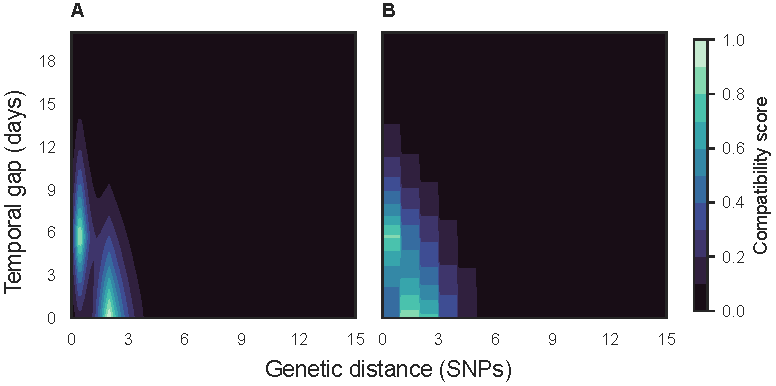
\includegraphics[width=0.8\textwidth]{figures/Fig2}
\caption{\textbf{EpiLink compatibility surfaces.}
Contour plots of EpiLink compatibility as a function of genetic distance (x-axis) and temporal gap (y-axis), using baseline inference parameters. (A) deterministic genetic component; (B) stochastic genetic component.}
\label{fig:surfaces}
\end{figure}

\subsection*{Baseline synthetic performance}

Our evaluation used a 4{,}990-node transmission tree yielding 12{,}447{,}555 scored pairs. We identified $10^{-4}$ as a reasonable sparsification threshold: at this cutoff, 87--97\% of edges were removed yet more than 99.8\% of total graph weight was preserved, reducing pipeline runtime from 38--62 seconds to 0.9--3.6 seconds per model (17--54$\times$ speed-up) with no meaningful effect on downstream community structure. We therefore applied this threshold in all subsequent clustering analyses.

In the baseline scenario, LD showed the strongest overall performance, achieving the highest average precision (AP = 0.568) and F1 score (0.688), while also maintaining high partition stability across Leiden resolution steps (mean = 0.895, SD = 0.044) (Table~\ref{tab:baseline}). LS produced lower discrimination than LD (AP = 0.275; F1 = 0.570), but had the highest mean partition stability overall (0.927), indicating especially robust partitions across clustering resolutions. Among the EpiLink variants, ESD performed best (AP = 0.469, F1 = 0.601, stability = 0.851). EDD and ESS showed intermediate F1 scores (0.556 and 0.534, respectively), while EDS had the weakest discrimination (AP = 0.090), despite still achieving F1 = 0.476 and mean stability = 0.834. Overall, weaker edge-level discrimination did not translate proportionally into uninformative clustering.

\begin{table}[!ht]
\caption{\textbf{Performance at baseline scenario.}}
\label{tab:baseline}
\begin{adjustbox}{max width=\textwidth}
\begin{tabular}{lcccc}
\toprule
Model & Average precision (AP) & BCubed F1 score & Mean partition stability (SD) \\
\midrule
EDD & 0.300 & 0.556 & 0.871 (0.077) \\
EDS & 0.090 & 0.476 & 0.834 (0.090) \\
ESD & 0.469 & 0.601 & 0.851 (0.073) \\
ESS & 0.190 & 0.534 & 0.830 (0.079) \\
LD  & 0.568 & 0.688 & 0.895 (0.044) \\
LS  & 0.275 & 0.570 & 0.927 (0.094) \\
\bottomrule
\end{tabular}
\end{adjustbox}
\end{table}

\subsection*{Consistency across perturbation scenarios}

The baseline performance ordering was consistent across all twelve perturbed scenarios (Fig.~\ref{fig:trend}). LD remained the top-performing model in discrimination and clustering accuracy under both matched and mismatched conditions, while ESD was the strongest-performing EpiLink variant across scenarios. EDS consistently showed the lowest AP, yet still yielded moderately coherent partitions, reinforcing the point that aggregating many noisy pairwise scores into a graph can still recover meaningful local transmission neighbourhoods. Overall, matched and mismatched conditions followed closely similar trajectories for AP, F1, and partition stability, though as described below, the mismatched condition revealed substantially greater losses in specific scenarios.

\begin{figure}[hp]
\centering

\includegraphics[width=0.8\textwidth]{figures/Fig3}
\caption{\textbf{Overall performance across all six models.}
Performance metrics under matched (inference parameters updated to reflect each perturbed data-generation scenario) and mismatched (inference parameters held fixed at baseline; data-generation parameters varied) conditions, evaluated across all 12 perturbation scenarios plus the unperturbed baseline. (A) Average precision (AP). (B) Best F1 score across Leiden resolution sweep. (C) Mean resolution stability (F1 between consecutive Leiden resolution steps; measures robustness to the choice of resolution parameter). (D) SD of resolution stability. Error bars show the 95\% confidence interval.}
\label{fig:trend}
\end{figure}

\subsection*{Sensitivity to parameter misspecification}

Under the matched condition, F1 losses were generally smaller in magnitude than the corresponding AP losses (Fig~\ref{fig:sensitivity}, \nameref{par:S1_Fig}), with the majority of scenarios producing effects within $\pm0.10$ of baseline for all models, indicating that all six models maintain reasonable clustering performance when inference is appropriately adapted to the underlying process.

\begin{figure}[hp]
\centering

\includegraphics[width=0.8\textwidth]{figures/Fig4}
\caption{\textbf{Sensitivity of F1 performance to perturbations of data-generating
parameters.} Lollipop plot showing best-F1 loss relative to the unperturbed baseline for each model across twelve perturbation scenarios, under matched (blue) and mismatched (coral) inference conditions. Matched: inference parameters updated to reflect each perturbed scenario; mismatched: inference parameters held fixed at baseline. Each row corresponds to a perturbation scenario. Positive values indicate improved performance relative to baseline; negative values indicate degradation.}
\label{fig:sensitivity}
\end{figure}

The mismatched condition revealed substantially greater and more heterogeneous degradation. The most severe losses occurred under increased incubation CV, where all models suffered F1 reductions of 0.56--0.66---by far the largest effect
observed across any scenario. This asymmetric sensitivity was unique to the upward perturbation; reducing incubation CV produced minimal change under either condition. Reduced clock rate constituted the second major vulnerability, with F1 losses of 0.27, 0.15, and 0.13 for EDD, ESD, and EDS respectively, while LD and LS were comparatively unaffected (losses of approximately 0.11 and 0.02), consistent with these models not explicitly incorporating a molecular clock
assumption. Reduced incubation mean also produced notable mismatched degradation, particularly for EDD ($-$0.20) and EDS ($-$0.12), whereas increasing the incubation mean had little effect in either condition.

Perturbations to testing delay parameters produced consistently small F1 changes across all models and conditions, suggesting moderate misspecification of the testing delay distribution is relatively inconsequential for clustering performance. Similarly, clock relaxation scenarios had largely negligible effects, with the exception of a modest matched-condition loss for EDS under the strict clock scenario.

Across models, EDD showed the greatest overall sensitivity to mismatched perturbations, while LD and LS exhibited the most consistently robust performance. Stochastic input models (EDS, ESS, LS) tended to show smaller degradations than
their deterministic-input counterparts (EDD, ESD, LD) in several mismatched scenarios. Taken together, these results identify incubation period variability and molecular clock rate as the primary sources of performance vulnerability under parameter misspecification.

\subsection*{Temporal stability of cumulative clustering}

Temporal stability was evaluated over 25 consecutive weekly transitions across the simulated epidemic (Fig~\ref{fig:stability}). In all models, instability was concentrated in the earliest epidemic weeks when case counts and cluster structure were sparse, with minimum Jaccard values occurring in weeks 1--3; stability rose rapidly thereafter and remained high for the remainder of the horizon. From week 3 onward, mean Jaccard indices ranged from 0.755 (EDS) to 0.926 (LS), with LS the only model that never fell below 0.7 across any transition. ESS showed the largest early instability spike, with a minimum Jaccard of 0.252, while LD and LS were the most consistently stable throughout. Mean forward and backward overlaps exceeded the Jaccard index for all models, reflecting the asymmetry
between new cases entering existing clusters and the persistence of earlier assignments---a pattern expected under cumulative case accumulation. Overall, all six models produced partitions that were largely stable and reproducible
across the simulated epidemic horizon, supporting their suitability for rolling surveillance.

\begin{figure}[hp]
\centering

\includegraphics[width=0.8\textwidth]{figures/Fig5}
\caption{\textbf{Temporal stability of cluster partitions as the epidemic accumulates.}
Forward overlap, backward overlap, and Jaccard index between consecutive weekly partitions, plotted against epidemic week. Stability is lowest in the first 1--2 epidemic weeks when cluster structure is sparse, rising rapidly and remaining high thereafter. LS is the only model that never falls below Jaccard = 0.7.}
\label{fig:stability}
\end{figure}

\subsection*{Application to empirical data recovers exposure-enriched clusters}

Applying EpiLink to 297{,}396 unique pairs from 772 Boston sequences yielded 77 clusters of size $\ge 2$, containing 642 sequences in total, with a highly right-skewed size distribution (median = 3, mean = 8.3, max = 84) (Fig~\ref{fig:boston}A). Five focus clusters contained at least one conference- or SNF-linked case, with exposure composition deviating significantly from background in all five ($\chi^2$, all $p < 0.003$) (Fig~\ref{fig:boston}B).

\begin{figure}[!htbp]
\centering
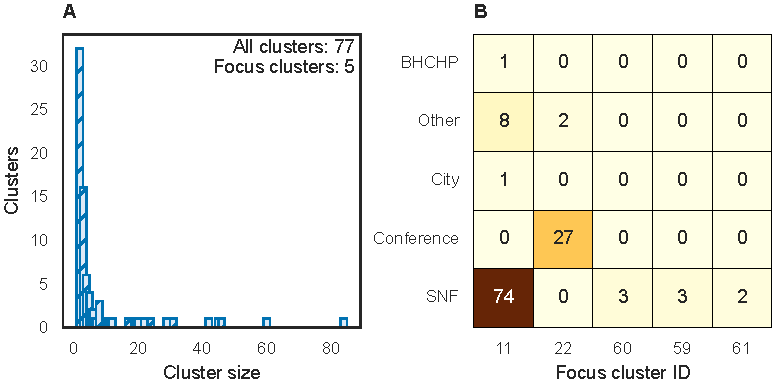
\includegraphics[width=0.8\textwidth]{figures/Fig6}
\caption{\textbf{EpiLink clustering of the Boston MGH/DPH SARS-CoV-2 dataset.}
(A) Distribution of Leiden cluster sizes across all 772 sequences; 5 of 77 clusters are annotated as focus clusters. (B) Heatmap of exposure category counts across the 5 focus clusters, annotated with raw case counts.}
\label{fig:boston}
\end{figure}

The two largest focus clusters illustrate the signal EpiLink recovers. Cluster 11 ($n = 84$) was dominated by SNF-linked cases (88.1\%), with mean intra-cluster SNP distance of 0.69 (max 4) and mean sampling gap of 2.3 days (max 6) --- consistent with a tight, contemporaneous outbreak. Cluster 22 ($n = 29$) was enriched for
conference-linked cases (93.1\%), with similarly compact genetic and temporal structure (mean SNP distance 1.14, max 5; mean gap 1.4 days, max 7). In both cases, mean inter-cluster SNP distance (5.0 for cluster 11) confirmed clear genetic separation from background. These results demonstrate that EpiLink recovers epidemiologically coherent clusters in real-world surveillance data, with cluster membership reflecting known exposure structure rather than sampling artefact.

\section*{Discussion}

This study introduces EpiLink as an interpretable, label-free alternative to threshold-based genomic clustering, replacing hard cut-offs with a graded measure of recent-transmission compatibility that makes its biological assumptions explicit. The results clarify both where this approach adds value and where its limitations lie.

The motivation for EpiLink arose partly from the challenge of superspreading events, in which rapid, clustered transmission produces many cases with minimal genetic divergence within a short time window, making it difficult to distinguish true transmission links from coincidental similarity on sequence data alone. The Boston application illustrates that this is tractable: EpiLink recovered clusters strongly enriched for the skilled nursing facility and conference outbreaks without any supervised training, and cluster membership reflected documented exposure
structure rather than sampling artefact. That result is precisely the operational context for which the method was designed---consensus genomes and case times available, transmission labels absent, and the goal a recoverable recent-transmission neighbourhood rather than a direction-resolved transmission tree.

The synthetic benchmark places that result in context. Under matched baseline conditions, the supervised logistic comparator LD achieved stronger pairwise discrimination and clustering accuracy. This is expected: a model trained on
labelled pairs has access to information EpiLink does not. The more relevant comparison is between EpiLink and the threshold-based approaches it is intended to replace. Within the EpiLink variants, the heterogeneity across EDD, EDS, ESD, and ESS is informative in its own right: each captures a distinct form of temporal--genetic model mismatch, and their relative performance indicates which sources of stochasticity most affect pairwise identifiability under a given
generating regime.

The misspecification analysis identifies incubation period variability and molecular clock rate as the primary practical vulnerabilities. The severe F1 losses under increased incubation CV in the mismatched condition reflect a fundamental identifiability problem: when infection-to-sampling intervals are highly variable and shorter, the temporal signal that EpiLink relies on becomes diffuse, and no amount of model adaptation fully recovers the lost resolution~\cite{Campbell2018a, VillabonaArenas2020, Duchene2020, Suster2022}. The comparative robustness of LD and LS to clock-rate perturbation---consistent with these models not incorporating an explicit molecular clock---suggests that when
substitution rates are uncertain or variable, model-agnostic supervised approaches may be preferable if training data are available. Testing delay misspecification, by contrast, had negligible effects, which is reassuring given that testing
behaviour is often poorly characterised in real surveillance.

Temporal stability results support use in a rolling surveillance setting. Once cumulative case counts grew beyond the first two to three weeks, cluster assignments were largely preserved across consecutive weekly updates for all models. The early instability is an artefact of sparse case accumulation rather than intrinsic model fragility, and the asymmetry between forward and backward overlap reflects the expected structure of case accumulation: new cases enter existing clusters (high backward overlap) before those clusters are fully resolved.

Several limitations deserve acknowledgement. EpiLink operates on consensus genomes and therefore ignores within-host diversity and minority variants that may carry additional transmission signal. The target scenario set
$\mathcal{S}_\star$ must be specified by the user; the default restriction to direct transmission and co-primary infection is appropriate for recent linkage but would miss longer transmission chains. Compatibility scores are not
calibrated posterior probabilities, and downstream clustering performance depends on the Leiden resolution parameter in ways that require careful sensitivity analysis, even though it remains generally robust to a broad range of permissible resolutions. Finally, the synthetic benchmark used a fixed transmission tree; performance on outbreak topologies with different heterogeneity profiles may differ.

Taken together, these results suggest a practical positioning for EpiLink within genomic epidemiology. When labelled training data are abundant and transferable to the setting of interest, supervised models will often achieve stronger
pairwise discrimination. EpiLink is most valuable when labels are unavailable, when analysts need to explain why a pair or cluster has been flagged, or when the inferential target is recent linkage under superspreading conditions rather than maximal clustering accuracy. In those settings, the explicit encoding of natural-history uncertainty into a graded compatibility score offers a principled and interpretable alternative to the ad hoc distance thresholds that remain dominant in routine surveillance.

\section*{Supporting information}

\paragraph*{S1 Appendix.}
\label{par:S1_Appendix}
\textbf{Detailed derivation and modelling assumptions for the EpiLink compatibility model.}
Provides the full derivation of the scenario-specific testing-time difference and transmission-related branch length used by EpiLink, together with the natural-history, observation, and molecular-clock assumptions.

\paragraph*{S1 Fig.}
\label{par:S1_Fig}
\textbf{Sensitivity of average precision (AP) to perturbations of data-generating parameters.}
Lollipop plot showing AP loss relative to the unperturbed baseline for each model across twelve perturbation scenarios, under matched (blue) and mismatched (coral) inference conditions. Matched: inference parameters updated to reflect each perturbed scenario; mismatched: inference parameters held fixed at baseline. Each row corresponds to a perturbation scenario. Positive values indicate improved performance relative to baseline; negative values indicate degradation. Arrows indicate values exceeding the axis range.

\section*{Acknowledgements}
This research was funded in whole, or in part, by the Wellcome Trust [Grant number 218471/Z/19/Z]. For the purpose of open access, the author has applied a CC BY public copyright licence to any Author Accepted Manuscript version arising from this submission.

\section*{Competing interests}
The authors have declared that no competing interests exist.

\nolinenumbers

\bibliographystyle{plos2015}
\bibliography{references}

\end{document}
